\documentclass[tikz,border=2pt]{standalone}
\usepackage{amsmath,amssymb}
\usepackage{pgfplots}
\pgfplotsset{compat=1.18}

\begin{document}
% (1 + x/n)^n for n = 1, 2, 5, 20 against e^x: the curves rise to the exponential as n grows.
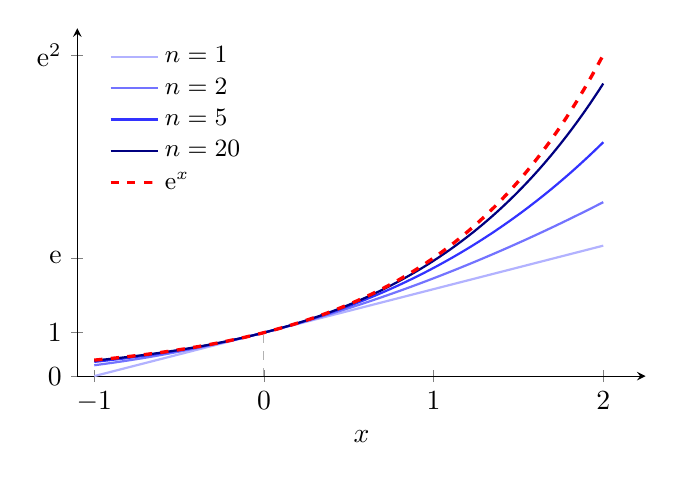
\begin{tikzpicture}
	\begin{axis}[
		axis lines=left, xmin=-1.1, xmax=2.25, ymin=0, ymax=8,
		xtick={-1,0,1,2}, ytick={0,1,2.718,7.389}, yticklabels={$0$,$1$,$\mathrm{e}$,$\mathrm{e}^2$},
		xlabel={$x$},
		samples=120, smooth, width=8.8cm, height=6cm, clip=false,
		legend style={draw=none, fill=none, font=\small, at={(0.04,0.98)}, anchor=north west}, legend cell align=left
		]
		\addplot[blue!30, thick, domain=-1:2] {1+x};
		\addlegendentry{$n=1$}
		\addplot[blue!55, thick, domain=-1:2] {(1+x/2)^2};
		\addlegendentry{$n=2$}
		\addplot[blue!80, thick, domain=-1:2] {(1+x/5)^5};
		\addlegendentry{$n=5$}
		\addplot[blue!50!black, thick, domain=-1:2] {(1+x/20)^20};
		\addlegendentry{$n=20$}
		\addplot[red, very thick, dashed, domain=-1:2] {exp(x)};
		\addlegendentry{$\mathrm{e}^x$}
		\draw[gray!60, dashed] (axis cs:0,0) -- (axis cs:0,1);
	\end{axis}
	
\end{tikzpicture}
\end{document}
